% =====================================================================
\chapter{Exécution, couverture et architecture logicielle}
\label{ch:15}
% =====================================================================

\section{Objectifs et organisation du chapitre}

\paragraph{Objectifs.} Le dépôt \texttt{atjte} contient beaucoup plus de code d'exécution que de code de signal : c'est la réalité de l'arbitrage entre plateformes. À la fin du chapitre, vous saurez : (1) identifier le risque de jambe et le quantifier ; (2) expliquer la sélection adverse d'un ordre \emph{maker} couvert sur une autre plateforme ; (3) mesurer l'effet du retard de recotation et de la latence de couverture ; (4) choisir sur quelle plateforme coter ; (5) concevoir une architecture qui survive aux pannes, aux déconnexions et aux erreurs humaines.

\paragraph{Code.} \texttt{code/ch15/ch15\_execution.py}.

% =====================================================================
\section{Le risque de jambe}
% =====================================================================

Un trade de paire comporte deux ordres sur deux instruments, souvent sur deux plateformes. Ils ne sont jamais exécutés exactement au même instant ni au prix prévu. Entre les deux exécutions, le prix bouge : c'est le \emph{risque de jambe} (\emph{leg risk}). Dans le pire des cas, une jambe est exécutée et l'autre est refusée (déconnexion, marge insuffisante, marché fermé) : on se retrouve avec une position directionnelle non voulue.

\begin{proposition}\label{c15:prop:leg}
Si le prix suit une marche aléatoire de volatilité $\sigma$ par unité de temps et que les deux exécutions sont séparées d'un délai $\Delta$, l'écart réalisé diffère de l'écart visé d'une quantité d'espérance nulle et d'écart-type $\sigma\sqrt\Delta$.
\end{proposition}
\begin{proof}
C'est la proposition~\ref{c1:prop:rw} appliquée sur la durée $\Delta$ : l'accroissement d'une marche aléatoire sur $\Delta$ unités de temps a une variance $\sigma^2\Delta$.
\end{proof}

\begin{codebox}[ — E3, risque de jambe d'une exécution taker-taker (or, volatilité 15\,\% par an)]
Écart-type de l'écart réalisé : $0{,}06$ pb pour un décalage de 10 ms, $0{,}20$ pb pour 100 ms, $0{,}62$ pb pour 1 s, $1{,}38$ pb pour 5 s (conformes à $\sigma\sqrt\Delta$) ; quantile 1\,\% : $-1{,}4$ pb à 1 s et $-3{,}2$ pb à 5 s. Pour une cryptomonnaie de volatilité 60\,\%, tous ces nombres sont multipliés par 4.
\end{codebox}

Le risque de jambe est d'espérance nulle si le délai est indépendant des mouvements de prix. Il devient un coût quand il ne l'est pas, ce qui est précisément le cas des ordres \emph{maker}.

% =====================================================================
\section{La sélection adverse d'un ordre \emph{maker}}
% =====================================================================

\subsection{Le mécanisme}

Une stratégie \emph{maker-taker} (comme celle d'\texttt{atjte}) affiche un ordre limite sur la plateforme A à un prix calculé à partir de la plateforme de référence B, attend d'être exécutée, puis couvre immédiatement sur B au marché. Le prix affiché doit être recalculé à chaque mouvement de B. Si la recotation a du retard, l'ordre affiché devient \og périmé\fg{} : quand B baisse, notre prix d'achat sur A reste trop haut un instant, et c'est précisément à ce moment que quelqu'un vient nous vendre. On est exécuté quand on a tort.

\begin{intuition}
Vous affichez dans votre vitrine un prix d'achat pour de l'or, calculé d'après le cours de ce matin. Si le cours chute à midi et que vous ne changez pas l'étiquette, tous les vendeurs du quartier viennent chez vous. Vous ferez beaucoup d'affaires, toutes mauvaises.
\end{intuition}

\subsection{Expérience}

\begin{codebox}[ — E1 et E2, glissement d'un achat maker couvert]
\textbf{Protocole :} prix de l'or simulé au pas de 50 ms pendant 4 heures ; la plateforme A suit B avec 200 ms de retard (E1) ou la précède de 200 ms (E2), avec un bruit de base ; ordre d'achat maker sur A à $1{,}2$\,\$ sous le prix acheteur de B ; couverture par une vente au prix acheteur de B. Le glissement mesure l'écart réalisé moins l'écart visé (négatif : perte). Environ 1\,900 exécutions par configuration. \textbf{Résultats} (glissement moyen, pb) :
\begin{center}\small
\begin{tabular}{lcccccc}
\toprule
 & \multicolumn{3}{c}{A suit B} & \multicolumn{3}{c}{A précède B}\\
\cmidrule(lr){2-4}\cmidrule(lr){5-7}
Retard de recotation & couv. 50 ms & 500 ms & 2 s & 50 ms & 500 ms & 2 s\\
\midrule
0 ms & $0{,}00$ & $0{,}00$ & $+0{,}02$ & $-0{,}01$ & $-0{,}13$ & $-0{,}11$\\
100 ms & $0{,}00$ & $0{,}00$ & $+0{,}01$ & $-0{,}02$ & $-0{,}13$ & $-0{,}13$\\
500 ms & $-0{,}15$ & $-0{,}16$ & $-0{,}14$ & $-0{,}09$ & $-0{,}21$ & $-0{,}20$\\
2 s & $-0{,}47$ & $-0{,}48$ & $-0{,}50$ & $-0{,}38$ & $-0{,}51$ & $-0{,}51$\\
\bottomrule
\end{tabular}
\end{center}
\end{codebox}

\begin{figure}[h]
\centering
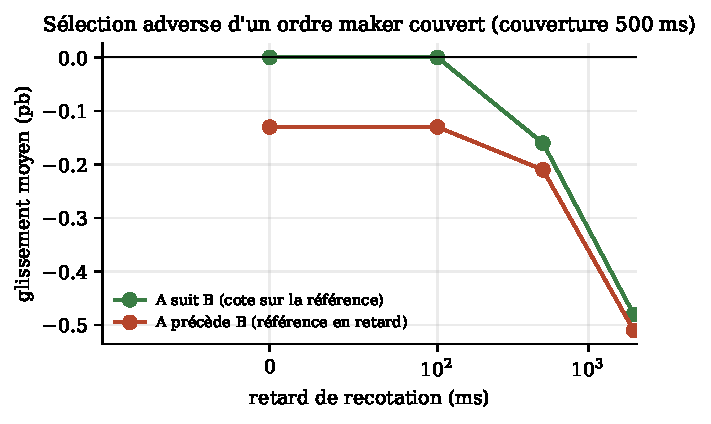
\includegraphics[width=0.66\textwidth]{ch15/selection_adverse.pdf}
\caption{Glissement moyen d'un achat maker couvert en fonction du retard de recotation, selon que la plateforme où l'on cote suit ou précède la référence.}
\label{c15:fig:adverse}
\end{figure}

\paragraph{Lecture.} (1) Tant que l'on recote vite et que l'on cote sur la plateforme \emph{suiveuse} (A suit B), le glissement est nul : notre prix bouge avant que le marché de A ne vienne le chercher. (2) Un retard de recotation de 2 s coûte environ $0{,}5$ pb par exécution, soit près d'un sixième d'un avantage visé de 3 pb. (3) Si l'on cote sur la plateforme \emph{meneuse} (A précède B), on est en retard par construction : même avec une recotation instantanée, la couverture sur B arrive après le mouvement. (4) Ces chiffres sont calculés pour l'or ; ils sont proportionnels à la volatilité et à la racine du retard, donc environ quatre fois plus grands pour une cryptomonnaie. Mesurer la relation meneur-suiveur entre ses deux plateformes (corrélation des variations décalées) est un préalable à toute stratégie maker-taker.

% =====================================================================
\section{Architecture : leçons d'\texttt{atjte}}
% =====================================================================

Le dépôt \texttt{atjte} \citep{atjte} illustre les choix d'architecture qu'impose une stratégie réelle. Les éléments suivants sont décrits dans sa documentation et son code.

\begin{description}
\item[Passerelles (\emph{gateways}).] Chaque plateforme est atteinte par un processus séparé qui détient seul les clés et les connexions ; les robots ne voient jamais de clé et passent par la passerelle en local. Une erreur dans un robot ne peut pas fuiter une clé ni ouvrir une connexion non contrôlée.
\item[Contrôle du ratio.] Le ratio $k$ (unités MT5 par unité de la plateforme) est vérifié au démarrage et en continu contre le rapport des prix, avec une tolérance de $\pm10\,\%$ : une erreur d'unité (facteur 10, inversion, onces contre grammes) est bloquée avant de couvrir dix fois trop ou trop peu.
\item[Seuils de couverture et lot minimal.] Une exposition inférieure au lot minimal du courtier ne peut pas être couverte ; le code avertit quand le seuil de couverture représente plus de deux lots minimaux, cas où une exposition significative resterait non couverte.
\item[Réconciliation.] La couverture et les contrôles portent sur l'exposition réelle relue sur les deux plateformes, pas sur le registre interne du robot ; un écart est vérifié une seconde fois avant correction, pour ne pas réagir à un état transitoire.
\item[Flux temps réel obligatoires.] Si le flux de prix est périmé ou si le flux des exécutions n'est pas confirmé, le robot annule ses ordres et se met en sommeil plutôt que de coter sur des données anciennes.
\item[Un robot par contrat.] Toutes les stratégies d'un même contrat partagent la position et le livre de couverture ; le démarrage est refusé si un autre robot est actif sur le même contrat.
\item[Mode simulation.] Rien n'est envoyé tant que \texttt{LIVE\_TRADING} n'est pas explicitement activé.
\item[Journalisation.] L'état du compte, les exécutions et l'historique de l'écart sont écrits en continu sur disque, pour reconstruire après coup ce qui s'est passé.
\end{description}

\begin{pitfall}
Chacun de ces mécanismes répond à un incident possible : couverture dans la mauvaise unité, exposition résiduelle sous le lot minimal, double robot sur le même compte, ordre envoyé sur une donnée vieille de dix secondes, plateforme qui ne confirme pas une exécution. Le dépôt rappelle lui-même qu'il a été écrit en grande partie avec des assistants de programmation et n'a pas été audité. Avant de confier de l'argent à un code, quel qu'il soit, lisez-le, testez-le en simulation, puis avec de petites tailles.
\end{pitfall}

\subsection{Liste de contrôle d'un moteur d'exécution}

\begin{enumerate}
\item Identifiants d'ordre uniques côté client, pour qu'un ordre renvoyé après une coupure ne soit pas exécuté deux fois.
\item Limitation du débit des requêtes (seau à jetons) pour respecter les quotas des plateformes.
\item Annulation automatique des ordres si le robot cesse de donner signe de vie (\emph{dead man's switch}), côté plateforme quand elle le propose.
\item Limites de risque indépendantes du signal : position maximale, perte journalière maximale, exposition non couverte maximale, plages horaires interdites (annonces, ouverture et maintenance des marchés).
\item Persistance de l'état et reprise propre après redémarrage.
\item Surveillance et alertes (téléphone) en cas d'écart de réconciliation, de rejet d'ordre ou de flux muet.
\end{enumerate}

% =====================================================================
\section{Ce que la théorie apporte, et ses limites}
% =====================================================================

\paragraph{Apports.} Une quantification du risque de jambe ($\sigma\sqrt\Delta$), une compréhension mécanique de la sélection adverse, et un critère pour choisir où coter (sur la plateforme suiveuse, avec une recotation rapide).

\paragraph{Limites.} Le modèle ignore la file d'attente (on n'est pas forcément servi au premier passage du prix), les exécutions partielles, les rejets, les pannes et la profondeur des carnets. Seuls des journaux d'exécution réels permettent de mesurer la sélection adverse effective.

% =====================================================================
\section{Fiche à recopier au tableau blanc}
% =====================================================================

\begin{whiteboard}
\begin{itemize}[leftmargin=1.2em]
\item \textbf{Risque de jambe :} écart-type $\sigma\sqrt\Delta$ ; nul en espérance seulement si le délai est indépendant des prix.
\item \textbf{Sélection adverse :} un ordre maker est exécuté quand le marché lui donne tort ; coût croissant avec le retard de recotation.
\item \textbf{Où coter :} sur la plateforme suiveuse ; couvrir sur la meneuse.
\item \textbf{Architecture :} passerelles, contrôle du ratio, lot minimal, réconciliation sur positions réelles, sommeil si flux périmé, un robot par contrat, mode simulation, journaux.
\end{itemize}
\end{whiteboard}

% =====================================================================
\section{Exercices}
% =====================================================================

\begin{exercise}
Une cryptomonnaie a une volatilité annuelle de 70\,\% (365 jours de 24 h). Calculez l'écart-type du risque de jambe pour un décalage de 300 ms.
\end{exercise}

\begin{exercise}
Pourquoi le glissement de E1 est-il légèrement positif pour une couverture à 2 s quand A suit B ? (Indice : que fait le bruit de base de A entre l'exécution et la couverture ?)
\end{exercise}

\begin{exercise}[à coder]
Ajoutez à E1 une file d'attente : on n'est exécuté que si le prix de A passe au moins 0,1\,\$ sous notre prix. Comment changent le nombre d'exécutions et le glissement ?
\end{exercise}

\begin{exercise}[données réelles]
Enregistrez pendant une journée les prix milieux de l'or sur deux plateformes au pas de la seconde. Calculez la corrélation entre les variations de l'une et les variations décalées de l'autre pour des décalages de $-5$ à $+5$ s. Laquelle mène ?
\end{exercise}

% =====================================================================
\section{Pour aller plus loin}
% =====================================================================

\begin{toread}
\begin{itemize}[leftmargin=1.2em]
\item \citet{harris2003} : les chapitres sur les fournisseurs de liquidité et la sélection adverse.
\item \citet{budish2015} : pourquoi les cotations périmées sont \og attrapées\fg{} par les plus rapides.
\item Le code d'\texttt{atjte} \citep{atjte} : \texttt{engines/arb/arb\_bot.py} (boucle principale, couverture, réconciliation), \texttt{engines/common/hedge\_gate.py} et \texttt{ratio.py}, \texttt{gateways/}.
\end{itemize}
\end{toread}

\section{Scripts du chapitre}
\noindent\texttt{code/ch15/ch15\_execution.py} : E1–E2 (figure~\ref{c15:fig:adverse}), E3.
